\subsection{Datasets used} \label{s:lit:datasets_used}

There are two important types of datasets used in the project: the gene expression on non-cancerous bladder from \acrfull{jbu} and MIBC cohort from \acrfull{tcga}. The JBU data, currently in the process of getting published \footnote{In the near feature after this PhD is completed, the data is likely to become available on a public portal}, helps build a representation of the urothelium that closely resembles the healthy tissue, which in this project is then used to inform the tumour stratification. The TCGA dataset is publicly available from the Genomics Data Central (GDC) portal\footnote{A new user needs to set an agreement with the GDC in order to have access \url{https://portal.gdc.cancer.gov/}}.


For both datasets the Kallisto method was used to align the RNA-seq reads using genome version GRCh38 with Gencode annotation version 42 which resulted in $\sim33k$ genes for each dataset.



\subsubsection*{The non-tumour dataset} \label{s:lit:non_tum_data}

Taking a bladder biopsy is an invasive procedure it is not possible to take samples from healthy patients, thus benign diseases were used to form a non-cancerous molecular representation of the bladder. These samples included \acrfull{oab}, \acrfull{sui}, \acrfull{nvh}, post-prolapse staging, survey after a \acrfull{tvt} procedure, and other abnormal conditions such as \acrfull{cc} and a patient suffering with \acrfull{ruti}.

The non-cancerous dataset from JBU comprised 88 samples, of which 49 are Abs-Ca differentiated, 23 are P0, and 14 are Undifferentiated (UD). The image in \cref{fig:lit:diff_samples} illustrates the different stages of tissue sample processing. After the biopsies are collected, the urothelium is separated from the stroma and the cells are segregated, resulting in freshly isolated cells or \acrshort{p0}. To obtain \acrfull{ud} cells, the protocol from \citet{Cross2005-fe} is used. To create a biomimetic tissue, the \acrshort{abs} differentiation protocol described by \citet{Cross2005-fe} is employed in the fourth step.

\begin{figure}[!htb]
    \centering
    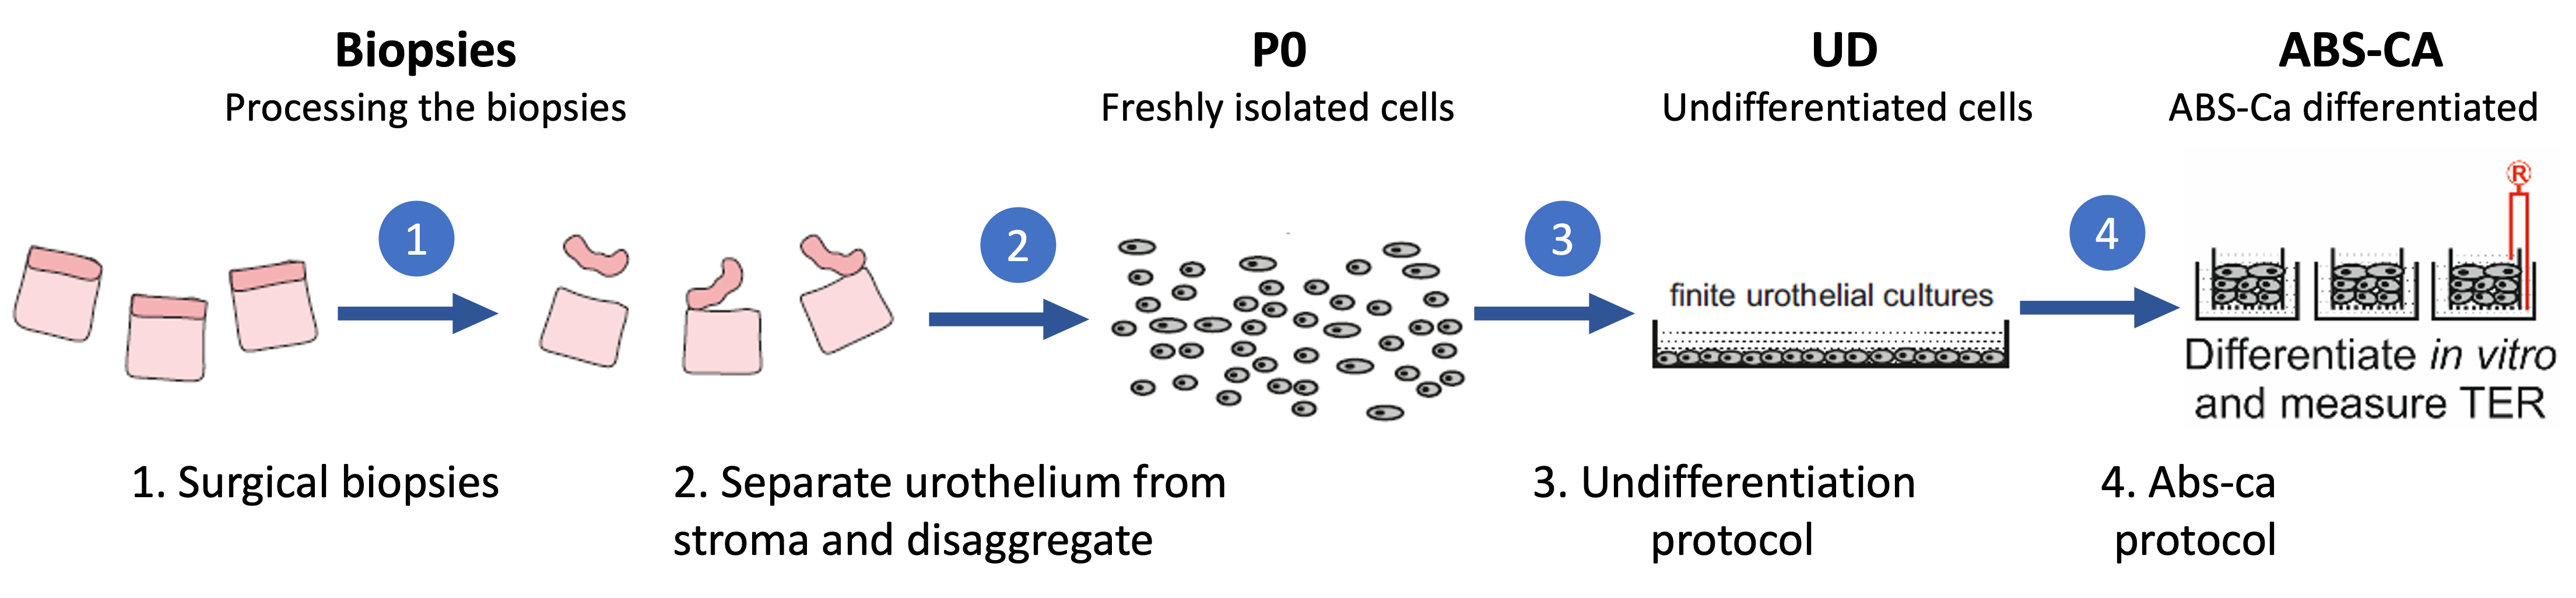
\includegraphics[width=1.0\textwidth, keepaspectratio]{Sections/Lit_review/Resources/differentiation.png}
    \caption{Overview of the processing of bladder tissue samples forming the non-tumour dataset from \acrfull{jbu}. After the collection of biopsies, the samples are processed to separate the urothelium from the stroma, resulting in freshly isolated cells (P0). To obtain undifferentiated cells, the protocol described by \citet{Cross2005-fe} is used. These cells can then be used to create biomimetic tissue using the Abs-Ca protocol described in \citet{Cross2005-fe}.}
    \label{fig:lit:diff_samples}
\end{figure}

% Aspects of the three differentiation status
The Abs-Ca samples were grown in the lab to exhibit the 'purer' markers of the urothelium differentiation and molecular properties of the healthy bladder tissue. The P0 samples exhibit the differentiation markers as in the Abs-Ca differentiated tissues as well as some cell infiltration aspects, offering a more realistic molecular representation of the bladder tissue. 

% Linking to the TCGA
By their differentiation status both Abs-Ca and P0 are closer to Luminal samples in the MIBC. The UD are on the other side of the differentiation spectrum and are closer to Basal MIBC subtypes. These aspects are observed in the analysis performed in the selective edge pruning, \cref{s:N_I:sel_pruning}, and in the work with the second version of the network pipeline in \cref{s:N_II:std_net}.

% Where this is used
In this project three different networks are created using the P0 and analysed in \cref{s:p0}, with the goal to inform the stratification of the \acrfull{mibc} using the molecular representation of freshly isolated cells. However, the P0 samples do not represent the Basal tumour samples which are closer to the  undifferentiated tissue state, and the research in \cref{s:N_II} utilised both the gene expressions from UD samples and the additional differentiated tissue samples with Abs-Ca.

\subsubsection*{The Cancer Genome Atlas} \label{s:lit:tcga_data}

The \acrshort{mibc} cohort from \acrfull{tcga} is central in this project, contributing with the gene expression from RNA-sequencing and the somatic mutations from Whole Exome Sequencing (WES) to all the results chapters.  The WES data was filtered and only non-synonymous mutations (Frameshift, Nonsense and Missense) are included as these have the potential to cause changes in the protein. The metadata available is used to compute the different survival rates for the subtypes derived across the project, see method in \cref{s:lit:survival}, and the cell infiltration analysis in \cref{fig:cs:tumour_purity}.








